\section{Example Using Two Hexahedra}
\label{sec:example:twohex8}

PyLith features discussed in this example:
\begin{itemize}
\item Quasi-static solution
\item Mesh ASCII format
\item Dirichlet boundary conditions
\item Kinematic fault interface conditions
\item Maxwell viscoelastic material
\item VTK output
\item Trilinear hexahedral cells
\item SimpleDB spatial database
\item ZeroDispDB spatial database
\item UniformDB spatial database
\item Filtering of cell output fields
\end{itemize}
All of the files necessary to run the examples are contained in the
directory \filename{examples/twocells/twohex8.}


\subsection{Overview}

This example is a simple 3D example of a quasi-static finite element
problem. It is a mesh composed of two trilinear hexahedra subject
to displacement boundary conditions. One primary difference between
this example and the example with two tetrahedra is that we use a
Maxwell viscoelastic material model, and run the model for 10 time
steps of 0.1 year each. Due to the simple geometry of the problem,
the mesh may be constructed by hand, using PyLith mesh ASCII format
to describe the mesh. In this example, we will walk through the steps
necessary to construct, run, and view three problems that use the
same mesh. In addition to this manual, each of the files for the example
problems includes extensive comments.


\subsection{Mesh Description}

The mesh consists of two hexahedra forming a rectangular prism (Figure
\vref{fig:twohex8-mesh}). The mesh geometry and topology are described
in the file \filename{twohex8.mesh}, which is in PyLith mesh ASCII format.

\begin{figure}
  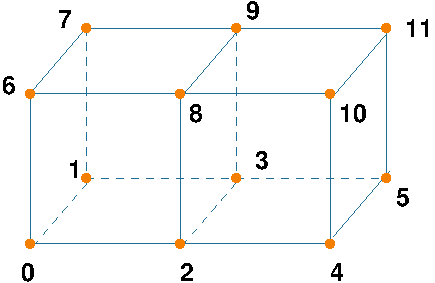
\includegraphics{examples/figs/twohex8-mesh}
  \caption{Mesh composed of two trilinear hexahedral cells used for
    the example problems.}
  \label{fig:twohex8-mesh}
\end{figure}


\subsection{Additional Common Information}

In addition to the mesh, the three example problems share additional
information, which we place in \filename{pylithapp.cfg}. Note that in
this example we make use of the UniformDB spatial database, rather
than the SimpleDB implementation used to specify the physical properties
in the other example problems. For simple distributions of material
properties (or boundary conditions), this implementation is often
easier to use. Examining \filename{pylithapp.cfg}, we specify the material
information with the following set of parameters:
\begin{cfg}
<h>[pylithapp.timedependent.materials]</h>
<f>material</f> = pylith.materials.MaxwellIsotropic3D

<h>[pylithapp.timedependent.materials.material]</h>
<p>label</p> = viscoelastic material
<p>id</p> = 1
<f>db</f> = spatialdata.spatialdb.UniformDB
<p>db.values</p> = [vp, vs, density, viscosity]
<p>db.data</p> = [5773.502691896258*m/s, 3333.333333333333*m/s, 2700.0*kg/m**3, 1.0e18*Pa*s]

<f>quadrature.cell</f> = pylith.feassemble.FIATLagrange
<p>quadrature.cell.dimension</p> = 3
\end{cfg}

\subsection{Axial Displacement Example}

The first example problem is extension of the mesh along the long
axis of the prism. Parameter settings that override or augment those
in \filename{pylithapp.cfg} are contained in the file \filename{axialdisp.cfg}.
These settings include:
\begin{inventory}
  \facilityitem{pylithapp.timedependent.bc.x\_neg}{Defines which degrees of freedom
    are being constrained (x, y, and z), gives the label (\facility{x\_neg},
    defined in \filename{twohex8.mesh}) defining the points desired, assigns
    a label to the boundary condition set, and gives the name of the spatial
    database with the values for the Dirichlet boundary conditions (\filename{axialdisp.spatialdb}).}
  \facilityitem{pylithapp.timedependent.bc.x\_pos}{Defines which degrees of freedom
    are being constrained (x, y, and z), gives the label (\facility{x\_pos},
    defined in \filename{twohex8.mesh}) defining the points desired, assigns
    a label to the boundary condition set, and gives the name of the spatial
    database with the values for the Dirichlet boundary conditions (\filename{axialdisp.spatialdb}).}
  \facilityitem{pylithapp.timedependent.materials.material.output}{Defines the
    filter to be used when writing cell state variables (average over
    the quadrature points of the cell), specifies which state variables
    and properties to output, gives the base filename for state variable
    output files, and defines the format to use when defining the output
    filenames for each time step.}
\end{inventory}
The values for the Dirichlet boundary conditions are given in the
file \filename{axialdisp.spatialdb}, as specified in \filename{axialdisp.cfg}.
Since data are being specified using two control points (rather than
being uniform over the mesh, for example), the data dimension is one.
Note that since we are using a Maxwell viscoelastic model, we request
that additional state variables and properties be output:
\begin{cfg}
<h>[pylithapp.timedependent.materials.material.output]</h>
<p>cell_data_fields</p> = [total_strain, viscous_strain, stress]
<p>cell_info_fields</p> = [mu, lambda, density, maxwell_time]
\end{cfg}
The files containing common information (\filename{twohex8.mesh},
\filename{pylithapp.cfg}) along with the problem-specific files
(\filename{axialdisp.cfg}, \filename{axialdisp.spatialdb}) provide a
complete description of the problem, and we can then run this example
by typing
\begin{shell}
$ pylith axialdisp.cfg
\end{shell}
Once the problem has run, two sets of files will be produced, along
with one additional file. The first set will have filenames such as
\filename{axialdisp\_txxxx.vtk}, where \filename{xxxx} is the time for
which output has been produced. In \filename{axialdisp.cfg} we specify
that the time stamp should be normalized by a value of 1.0 years and
the time stamp should be of the form \filename{xxx.x} (recall that the
decimal point is removed in the filename). As a result, the filenames
contain the time in tenths of a year. These files will contain mesh
information as well as displacement values for the mesh vertices at
the given time. The second set of files will have names such as
\filename{axialdisp-statevars\_txxxx.vtk}, where \filename{xxxx} is
the time in tenths of a year (as above) for which output has been
produced. These files contain the state variables for each cell at the
given time. The default fields are the total strain and stress fields;
however, we have also requested the viscous strains. As specified in
\filename{axialdisp.cfg}, these values are averaged over each
cell. The final file (\filename{axialdisp-statevars\_info.vtk}) gives
the material properties used for the problem. We have requested all of
the properties available for this material model (\texttt{mu},
\texttt{lambda}, \texttt{density}, \texttt{maxwell\_time}). If the
problem ran correctly, you should be able to produce a figure such as
Figure \vref{fig:twohex8-axial}, which was generated using ParaView.

\begin{figure}
  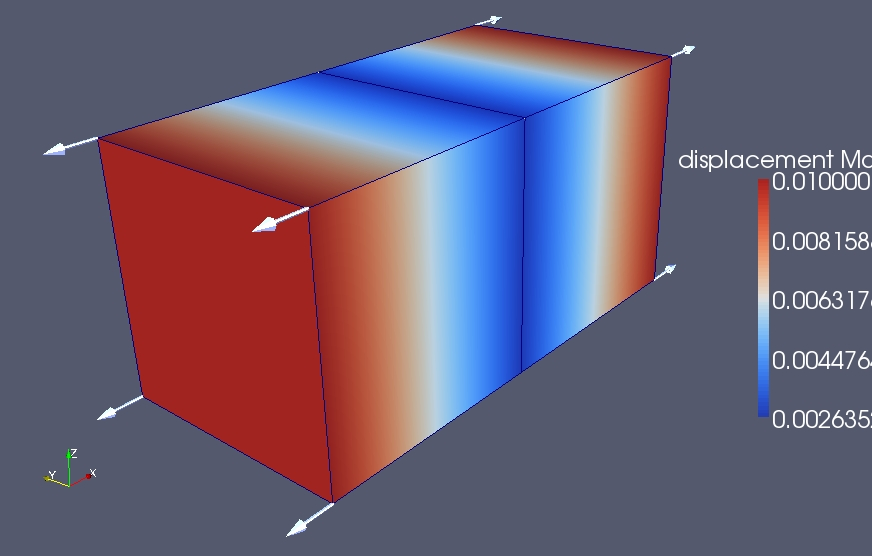
\includegraphics[scale=0.33]{examples/figs/twohex8-axialdisp}
  \caption{Color contours and vectors of displacement for the axial displacement
    example using a mesh composed of two trilinear hexahedral cells.}
  \label{fig:twohex8-axial}
\end{figure}


\subsection{Shear Displacement Example}

The second example problem is shearing of the mesh in the y direction.
Parameter settings that override or augment those in \filename{pylithapp.cfg}
are contained in the file \filename{sheardisp.cfg}. These settings include:
\begin{inventory}
  \facilityitem{pylithapp.timedependent.bc.x\_neg}{Defines which degrees of freedom
    are being constrained (x, y, and z), gives the label (\facility{x\_neg},
    defined in \filename{twohex8.mesh}) defining the points desired, assigns
    a label to the boundary condition set, and gives the name of the spatial
    database with the values for the Dirichlet boundary conditions (\filename{sheardisp.spatialdb}).}
  \facilityitem{pylithapp.timedependent.bc.x\_pos}{Defines which degrees of freedom
    are being constrained (x, y, and z), gives the label (\facility{x\_pos},
    defined in \filename{twohex8.mesh}) defining the points desired, assigns
    a label to the boundary condition set, and gives the name of the spatial
    database with the values for the Dirichlet boundary conditions (\filename{sheardisp.spatialdb}).}
\end{inventory}
The values for the Dirichlet boundary conditions are given in the
file \filename{sheardisp.spatialdb}, as specified in \filename{sheardisp.cfg}.
Data are being specified at two control points (rather than being
uniform over the mesh, for example), so the data dimension is one.
The files containing common information (\filename{twohex8.mesh}, \filename{pylithapp.cfg})
along with the problem-specific files (\filename{sheardisp.cfg}, \filename{sheardisp.spatialdb})
provide a complete description of the problem, and we can then run
this example by typing
\begin{shell}
$ pylith sheardisp.cfg
\end{shell}
If the problem ran correctly, you should be able to generate a figure
such as Figure \vref{fig:twohex8-shear}, which was generated using
ParaView.

\begin{figure}
  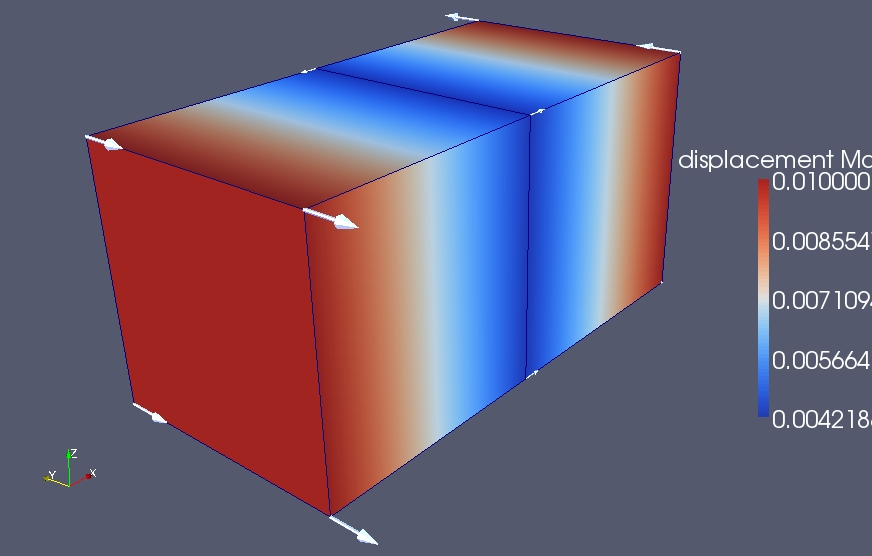
\includegraphics[scale=0.33]{examples/figs/twohex8-sheardisp}
  \caption{Color contours and vectors of displacement for the shear displacement
    example using a mesh composed of two trilinear hexahedral cells.}
  \label{fig:twohex8-shear}
\end{figure}


\subsection{Kinematic Fault Slip Example}

The next example problem is left-lateral fault slip applied between
the two hexahedral cells using kinematic cohesive cells. The vertices
away from the fault are held fixed in the x, y, and z directions.
Parameter settings that override or augment those in \filename{pylithapp.cfg}
are contained in the file \filename{dislocation.cfg}. These settings
include:
\begin{inventory}
  \facilityitem{pylithapp.timedependent.bc.x\_neg}{Defines which degrees of freedom
    are being constrained (x, y, and z), gives the label (\facility{x\_neg},
    defined in \filename{twohex8.mesh}) defining the points desired, and
    assigns a label to the boundary condition set. In this case, we use
    the default spatial database (ZeroDispDB) for the Dirichlet boundary
    condition, which sets the displacements to zero.}
  \facilityitem{pylithapp.timedependent.bc.x\_pos}{Defines which degrees of freedom
    are being constrained (x, y, and z), gives the label (\facility{x\_pos},
    defined in \filename{twohex8.mesh}) defining the points desired, and
    assigns a label to the boundary condition set.}
  \facilityitem{pylithapp.timedependent.interfaces}{Gives the label (defined in
    \filename{twohex8.mesh}) defining the points on the fault, provides
    quadrature information, and then gives database names for material
    properties (needed for conditioning), fault slip, peak fault slip
    rate, and fault slip time.}
\end{inventory}
The fault example requires three additional database files that were
not needed for the simple displacement examples. The first file
(\filename{dislocation\_slip.spatialdb}) specifies 0.01 m of
left-lateral fault slip for the entire fault.  The data dimension is
zero since the same data are applied to all points in the set. The
default slip time function is a step-function, so we also must provide
the time at which slip begins. The elastic solution is associated with
advancing from $t=-dt$ to $t=0$, so we set the slip initiation time
for the step-function to 0 in
\filename{dislocation\_sliptime.spatialdb}.  The files containing
common information (\filename{twohex8.mesh}, \filename{pylithapp.cfg})
along with the problem-specific files (\filename{dislocation.cfg},
\filename{dislocation\_slip.spatialdb},
\filename{dislocation\_sliptime.spatialdb}) provide a complete
description of the problem, and we can then run this example by typing
\begin{shell}
$ pylith dislocation.cfg
\end{shell}
If the problem ran correctly, you should be able to generate a figure
such as Figure \vref{fig:twohex8-disloc}, which was generated using
ParaView.

\begin{figure}
  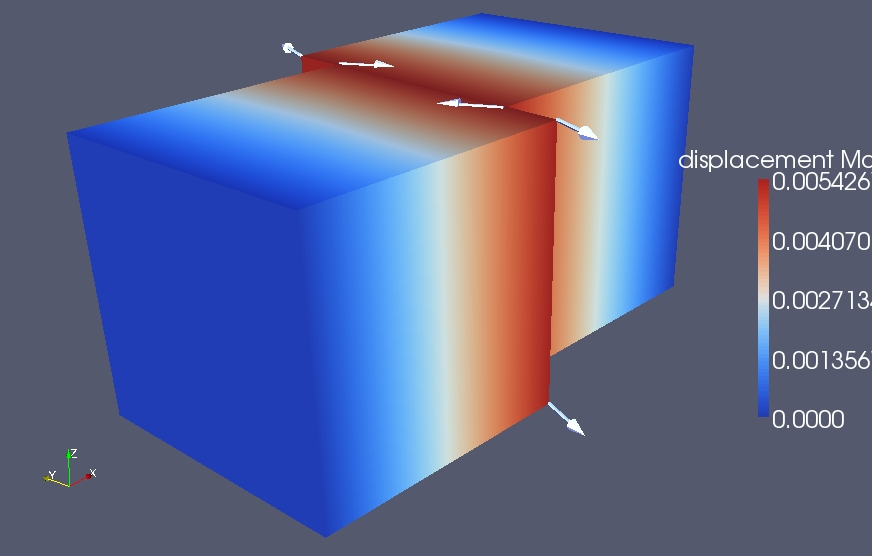
\includegraphics[scale=0.33]{examples/figs/twohex8-dislocation}
  \caption{Color contours and vectors of displacement for the kinematic fault
    example using a mesh composed of two trilinear hexahedral cells.}
  \label{fig:twohex8-disloc}
\end{figure}


% End of file
